\documentclass[preprint,5p,authoryear]{elsarticle}

\usepackage{amsmath}
\usepackage{amsfonts}
\usepackage{graphicx}
\usepackage[small]{caption}
\usepackage[subrefformat=parens]{subcaption}
\usepackage{booktabs}
\usepackage{multirow}
\usepackage{rotating}
\usepackage{url}
\usepackage[table]{xcolor}
\usepackage{hyperref}

\journal{NeuroImage}

\bibliographystyle{elsarticle-harv}

\begin{document}

\begin{frontmatter}

\title{Identifying Virtual World Induced Brain States using fMRI and Machine Learning}

\author[UT]{Andrew Floren\corref{cor}}
\ead{afloren@utexas.edu}

\author[UT]{Bruce Naylor}

\author[UT]{David Ress}

\address[UT]{The University of Texas at Austin, Austin, TX 78712 USA}

\cortext[cor]{Corresponding author.}

\begin{abstract}
abstract
\end{abstract}

\begin{keyword}
keyword1 \sep keyword2
\end{keyword}

\end{frontmatter}

\section{Introduction}
When conducting research using fMRI to analyze how the brain responds to visual stimuli, static images have been  the dominant choice.
While this has proven to be a successful approach, it does not mimic the dynamically changing environment in which brains have evolved.
It is reasonable to presume that the brain responds in a more complex manner to realistic conditions where the visual stimuli is very dynamic.
To capture these more complex aspects of brain activity requires a shift to dynamic stimuli.
We have taken a step towards this by employing virtual worlds, similar to what is commonly used in video games, to generate our visual stimuli in real-time.
This allows us to create as dynamic a stimuli as needed.
In addition, virtual worlds have two advantages over videos of the real world: 1) the scene designer has complete control over the stimuli 2) the subject can interact with the virtual world by making a sequence of decisions while in the scanner.

To analyze the brain response to our more complex stimuli, we felt that we needed to use a multi-voxel pattern recognition approach that identifies brain response patterns using all the voxels in a time-slice simultaneoulsy.
This is in contrast to utlizing the General Linear Model which treats each voxel independently as a time-series of responses over an entire multi-minute scan.
Multi-voxel pattern recognition \citep{Haxby2001,Mitchell2003,Haynes2006} involves the use of statistical machine learning algorithms, such as artificial neural networks and support vector machines.
When applying these algorithms to fMRI, the stimulus typically is organized into categories or classifications (e.g. houses, faces, tools etc.).
The machine learning algorihms use the fMRI data to synthsize models of the classes.
These models map a single fMRI time-slice to a set of weights, one for each category.
Each weight provides a prediction relative to the other weights that the time-slice corresponds to the brain responsing to stimuli from that category.
Comparing the highest predicted class to the known class gives a means of assessing the accuracy of the models.
Taking the next step of determining the importance of each voxel for selecting each class can be achieved by "inverting" the classifiers using a technique called "sensitivity analysis".
This gives an anatomical "importance map" for each category that can be displayed on an inflated cortex.
The net result is the familiar color-coded picture of a brain indicating the distribution of the brain response, but one that is computed very differently from GLM type techniques.

Given our long-term interest in PTSD, we created a virtual town for our stimulus intended to mimic the kinds of real-world settings encountered by our military forces.
Virtual characters representing friendly forces and hostile combatants were presented at a variey of locations thoughout the virtual town.
An animation was synthezied in real-time in which the camera moves at eye level throughout the town, stopping at various locations where a varying number and mix of characters where present.
Both the camera and the characters were animated at all times (no static imagery).
Instead of limiting the analysis to coarse categoires, such as friends vs. foes, we extented the analysis to the number of characters at each location.
This introduces to the experiment the identification of those parts of the brain involved in counting human-like characters.
We synthesized both linear SVMs (support vector machines) and feed forward neural networks to predict the number of characters.
The results were 3-4 times better than chance.

\section{Methods}

\subsection{Subjects}
Five male adults, with normal or corrected to normal vision, participated in the experiments. 
All subjects participated in three sessions, two sessions to collect machine-learning data, and one session to measure a high-resolution volume anatomy. 
Informed consent was obtained from all subjects.

\subsection{Stimulus}
We developed a virtual reality environment similar to many popular first person video games using the Unreal Engine 2 SDK \citep{UnrealEngine2}.
The stimuli is dynamically rendered and presented from the point of view of a camera moving through this virtual environment using a block design. 
First, the viewpoint moves for 15 seconds through the virtual environment with no characters present (Fig. \ref{fig:stimulus-movement}), then pauses for 15 seconds during which a group of characters fades into view (Fig. \ref{fig:stimulus-characters}). 
Each run consists of 12 alternations between moving through the virtual environment and character presentations. 
In each scanning session, 4 to 6 runs were collected.
\begin{figure*}
\centering
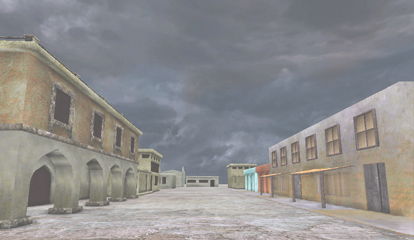
\includegraphics[width=0.8\textwidth]{figures/stimulus-movement}
\caption{An example frame from the stimulus while the camera is moving through the virtual envronment.}
\label{fig:stimulus-movement}
\end{figure*}
\begin{figure}
\centering
\begin{subfigure}{0.4\textwidth}
\centering
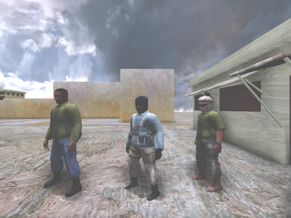
\includegraphics[width=\textwidth]{figures/stimulus-characters}
\caption{}
\label{fig:stimulus-characters}
\end{subfigure}
\begin{subfigure}{0.4\textwidth}
\centering
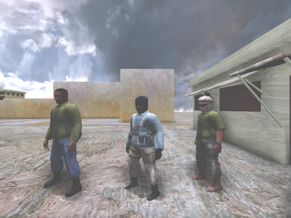
\includegraphics[width=\textwidth]{figures/stimulus-location}
\caption{}
\label{fig:stimulus-location}
\end{subfigure}
\caption{
\subref{fig:stimulus-characters} An example frame from the stimulus while characters are being presented.
\subref{fig:stimulus-location} Another example frame from the stimulus while characters are being presented.
Note how the locations of the characters varies considerably between these two frames.}
\label{fig:stimulus}
\end{figure}

The camera is constantly moving (even during the character presentation periods the camera slowly pans and rotates) and the characters are animated so that the presented scene is never static.
The number and location of characters varies with each presentation in a quasi-random fashion.
The number of characters presented varies from 1 to 6.
A presentation with a particular number of characters appears twice in each run, however the order of these presentations was randomized.
It should be noted that this random ordering was generated once and held constant between subjects.
Additionally, even between character presentations with the same number of characters, the locations of those characters varies considerably; compare figures \ref{fig:stimulus-characters} and \ref{fig:stimulus-location}.
[I need another frame from the stimulus to illustrate this point. These figures are all from the original report but I'd like to generate new ones if I can get access to a machine with the stimulus.]


\subsection{MRI protocols}
Imaging was performed an GE Signa Excite HD scanner using the product 8-channel head coil.
We collected whole-brain image volumes using a custom GRAPPA-accelerated EPI sequence \citep{newbold}. 
Sequence parameters were g-factor = 2,  TE = 25 ms, TR = 2.5 s, and  2.5-mm cubic voxels across a 200 mm field-of-view. 
The slice prescription included 40 slices oriented along the AC-PC axis. 
A high-order shim was  performed to improve field homogeneity.

A set of T1-weighted structural images was obtained on the same prescription at the end of each machine-learning session using a three-dimensional (3D) RF-spoiled GRASS (SPGR) sequence. 
These anatomical images were then used to align the functional data to a structural 3D reference volume, which was acquired for each subject in a separate session. 
The structural reference volume was T1-weighted with good gray-white contrast and was acquired using a 3D, inversion-prepared, SPGR sequence (minimum TE and TR, TI = 450 ms, 15° flip angle, isometric voxel size of 0.7 mm, 2 excitations, ~28-minimum duration).

\subsection{Preprocessing}
Preprocessing of the fMRI data was performed using the mrVista software package (available for download at \url{http://vistalab.stanford.edu/}) as well as additional tools developed on the mrVista framework in our lab. 
The first 15 seconds seconds of data  were discarded to reduce transient effects.
We then estimated in-scan motion using a robust scheme \citep{Nestares-and-Heeger-2000}. 
Between-run motion was corrected using the same intensity-based scheme, this time applied to the temporal average intensity of the entire scan. 
The last run of the session was used as the reference. 
Additionally, we applied a Wiener filter deconvolution \citep{Wiener} using a generic difference-of-gamma HRF \citep{Glover} to shift the peak response in time so that it is aligned with its associated stimulus.

Wiener filter deconvolution can be summarized as follows:
Given a system
\begin{equation}
y(t) = h(t) \ast x(t) + n(t)
\end{equation}
where $x(t)$ is the signal of interest, $h(t)$ is some blurring kernel, $n(t)$ is independent additive noise, and $y(t)$ is the recorded signal.
We want to find the deconvolution kernel $g(t)$ such that 
\begin{equation}
\hat{x}(t) = g(t) \ast y(t)
\end{equation}
minimizes the mean squared error between $x(t)$ and $\hat{x}(t)$, or
\begin{equation}
\sum_{t}{\left( \hat{x}(t) - x(t) \right)^{2}}
\end{equation}
The solution for the optimal $g(t)$ is most easily expressed in the Fourier domain.
\begin{equation}
g(t) \xrightarrow{\mathcal{F}} \frac{H^{*}(f)}{\left|H(f)^{2}\right| + \mbox{SNR}^{-1}(f)}
\end{equation}
Where $\mbox{SNR}(f)$ is the signal to noise ratio $\frac{\left| X(f) \right|}{\left| N(f) \right|}$.

In fMRI, $y(t)$ is the recorded BOLD signal, $h(t)$ is the hemodynamic response function, and $x(t)$ is the neuronal population response.
Calculating $g(t)$ requires estimates of the power spectral density of the signal of interest as well as the noise.
However, the noise $n(t)$ corresponds not only to scanner noise but other nuisance factors such as pulse and respiration.
This makes modeling the noise, and its power spectral density, very difficult.
Therefore, we set $\mbox{SNR}(f) = 1$ for all frequencies $f$.
Figure \ref{fig:wiener-deconvolution} illustrates the effects of this deconvolution on a simple square wave as well as an example voxel time series.

\begin{figure}
\centering
\begin{subfigure}{0.4\textwidth}
\centering
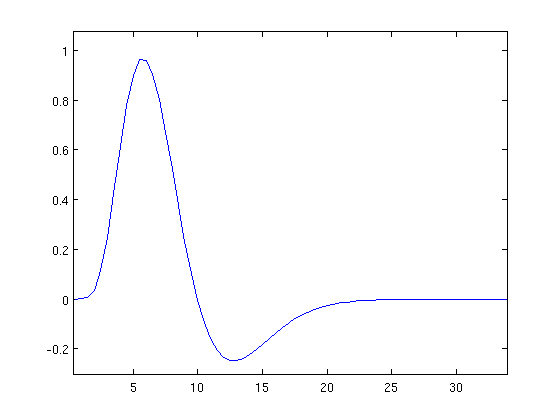
\includegraphics[width=\textwidth]{figures/hrf}
\caption{}
\label{fig:wiener-hrf}
\end{subfigure}
\begin{subfigure}{0.4\textwidth}
\centering
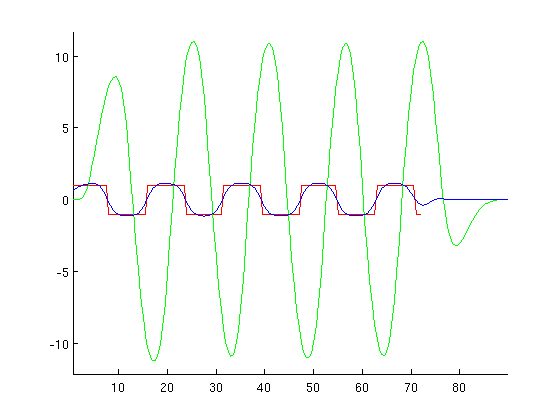
\includegraphics[width=\textwidth]{figures/wiener-square}
\caption{}
\label{fig:wiener-square}
\end{subfigure}
\begin{subfigure}{0.4\textwidth}
\centering
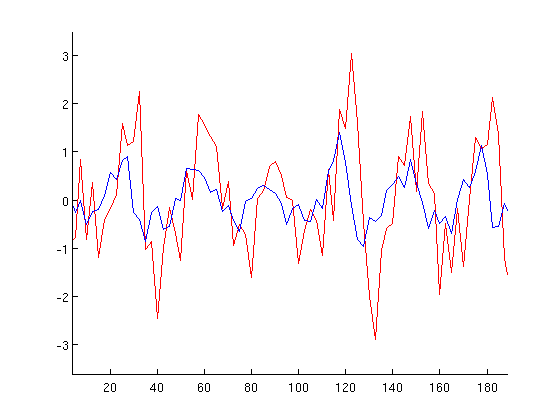
\includegraphics[width=\textwidth]{figures/wiener-voxel}
\caption{}
\label{fig:wiener-voxel}
\end{subfigure}
\caption{
\subref{fig:wiener-hrf} The difference-of-gamma HRF employed as $h(t)$. 
\subref{fig:wiener-square} A simple square wave in red. 
The same square wave after convolution with $h(t)$ in green, then after Wiener-filter deconvolution in blue. 
\subref{fig:wiener-voxel} An example voxel time series in red. 
The same time series after Wiener-filter deconvolution in blue.}
\label{fig:wiener-deconvolution}
\end{figure}

The high-resolution reference anatomies were segmented using the FreeSurfer analysis package \citep{FreeSurfer} to create approximate masks of the gray matter in each subject, as well as a surface model useful for visualization of the results.

\subsection{Dimensionality reduction}
We select a relevant subset of the volume using a harmonic power analysis based on the block design of our stimulus. 
One can show that the response of any linear system to a blocked alternation at frequency f will contain power only at f and its harmonics. 
Under a linear response assumption, we can therefore form an unbiased estimate of the response power by summing the power at these frequencies. 
Let $y(t)$ be the recorded discrete time series at some voxel.
Then let $Y(f)$ be the discrete Fourier transform of $y(t)$.
The fractional harmonic power of that time series is defined as:
\begin{equation}
P_h = \frac{\sum_{i = 1}^{M}{\left|Y(i \cdot N)\right|^{2}}}{\sum_{f}{\left|Y(f)\right|^{2}}}
\end{equation}
Where $P_h$ is the fractional harmonic power, $M$ is the number of harmonics, and $N$ is the frequency of interest, in our case the period of the block alternations. 
Because the BOLD response has a predominantly low-pass temporal frequency response, we chose $M = 4$. 
Using $P_h$, we then selected a particular number N (range 1000-3000) voxels with the greatest power. 

This harmonic-power selection was based on the alternation between characters present and characters absent, without regard to the number of characters presented. 
Therefore, we will only be presenting classifier accuracy estimates for character count, and not for the presence or absence of characters to avoid cross-contamination between dimension-reduction and  classification criteria that would result in inflated classifier performance estimates \citep{CrossContamination}.

\subsection{Classification}
Using the time series from the voxels selected by the harmonic power analysis, we trained a linear SVM and a feed forward neural network.
Generally, the performance of machine learning algorithms is estimated by splitting the available data into train and test sets and testing the performance of the algorithm on the test set after training on only the train set.
The algorithm's performance on the test set is an estimate of the classifier's performance on new data.
Certain iterative machine learning algorithms, such as neural networks, further subdivide the data into train, validate, and test sets.
The algorithm is trained on the training set and after each iteration is tested against the validation set.
When the performance on validation set stops improving, the algorithm stops iterating and is tested against the test set in order to estimate its performance.
We estimated the performance of our algorithms using a cross-fold approach \citep{Kohavi1995} where the data is split into folds which are used to form multiple train and test sets.

To maximize our temporal resolution, each frame (a point in the pre-processed time series) was treated as a separate data value, rather than of averaged across the block as has been done in previous work \citep{BlockAveraging}.
However, previous studies have discussed issues with optimistic performance estimates due to temporal correlations violating independence assumptions between training and test set examples \citep{Pereira2009}.
We were interested in more closely examining the relationship between performance estimates and this temporal correlation.
To accomplish this, we estimated classifier performance using 5 different methods for splitting the training and test examples in order to vary the average temporal delay between frames in the training and test sets. 
The first four methods deal only with frames from a particular session.
In the first method, which we will refer to as the frame split, frames were independently drawn into the training and test sets. 
Although the draws were independent, there is no restriction to prevent adjacent frames being split between the training and test sets.
In the second method, which we will refer to as the block split, sets of frames corresponding to the stimulus blocks were independently drawn into the training and test sets.
Our stimulus design enables us to break runs into two sets that each contain a complete set of character-number presentations. 
Accordingly, in our third method, which we will refer to as the half-run split, sets of frames were independently drawn from these half-runs. 
Similarly, in our fourth method, termed run split, entire runs of frames were independently drawn. 
For the fifth method, termed session split, we used one entire session for training and a second session for test.
This method is similar to measures of between-session classifier accuracy used previously \citep{BetweenSessionAccuracy}.
Table \ref{tab:training-split} summarizes these training and test set split methods and the mean temporal delay between the training and test data, which varies from $\sim$30 s (frame split) to several months (session split).

\begin{figure}
\centering
\begin{subfigure}{0.4\textwidth}
\centering
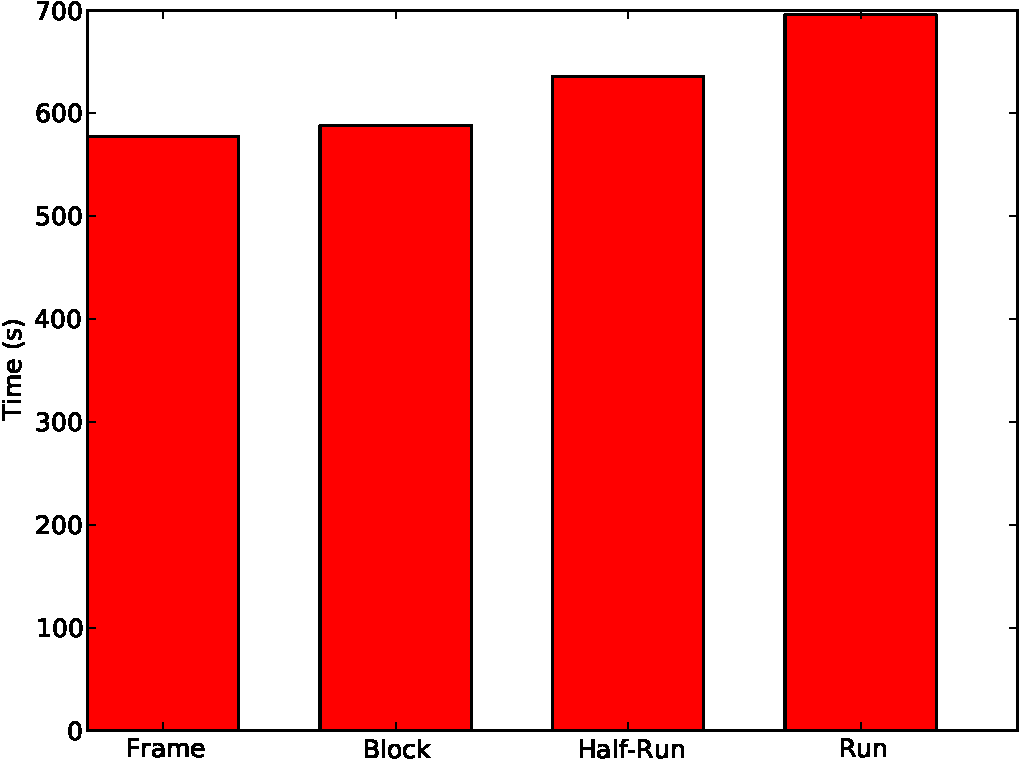
\includegraphics[width=\textwidth]{figures/mean-delay-graph}
\caption{}
\label{fig:mean-delay-graph}
\end{subfigure}
\begin{subfigure}{0.4\textwidth}
\centering
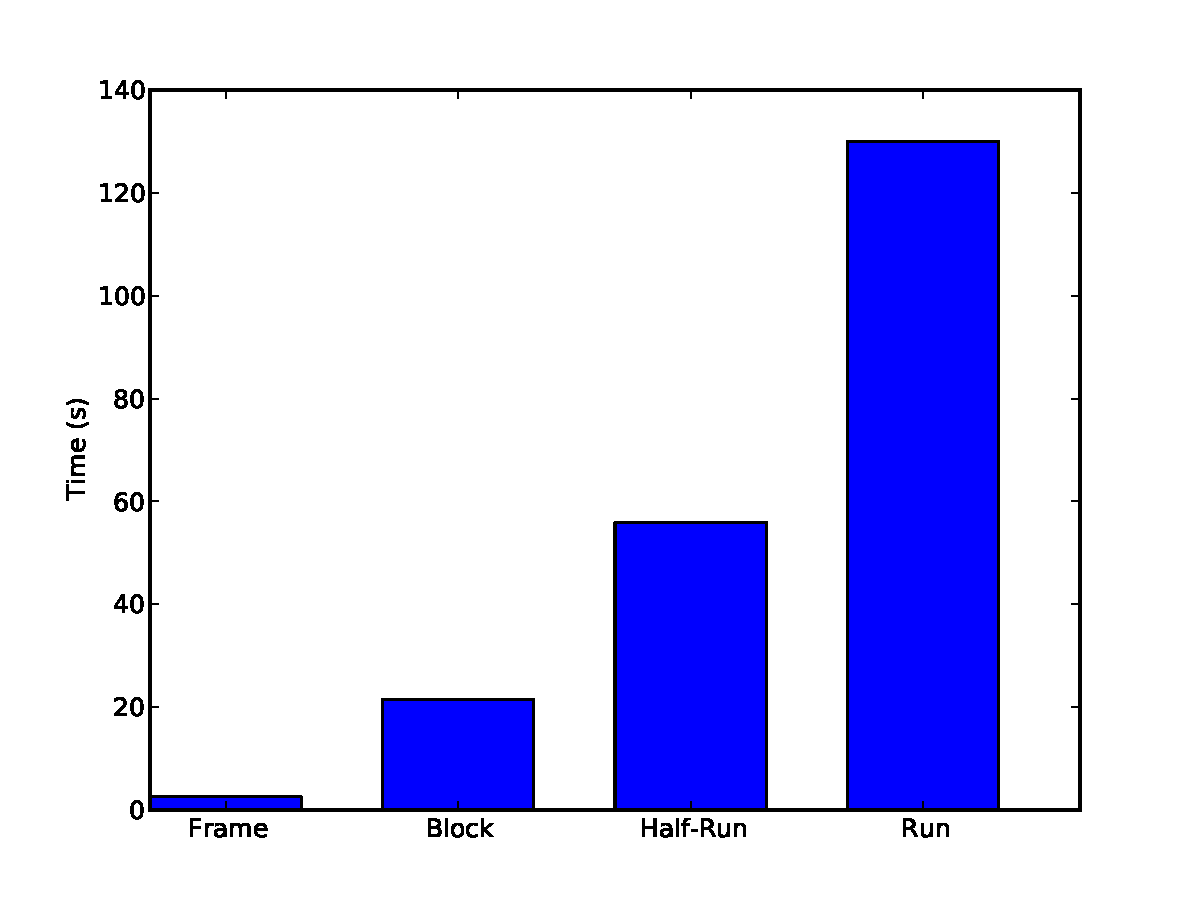
\includegraphics[width=\textwidth]{figures/min-delay-graph}
\caption{}
\label{fig:min-delay-graph}
\end{subfigure}
\caption{The \subref{fig:mean-delay-graph} mean delay and \subref{fig:min-delay-graph} minimum mean delay between examples in the train and test set for four of the split methods. 
The session split method is excluded because both the mean and minimum delay are much larger than the other splits and the delays vary significantly between subjects.}
\end{figure}

\begin{table}
\centering

\begin{tabular}{l*{2}{c}}
\toprule
Split & Mean Delay & Mean Minimum Delay \\
\midrule
Frame & 5776 & 26 \\
Block & 5883 & 215 \\
Half-Run & 6360 & 559 \\
Run & 6960 & 1300 \\
Session & 0 & 0 \\
\bottomrule 
\end{tabular}

\caption{Summary of training and test set split methods and the mean temporal delay between the training and test data.}
\label{tab:training-split}
\end{table}

For the frame and block splits, the classifier performances were estimated using 10-fold cross-validation.
That is, the dataset was randomly split into the training and test sets 10 times and a classifier is trained on each split.
The classifier's performance is then estimated as the average of its performance across all 10 splits.
For the half-run, run, and session splits, only 8, 4, and 2 unique splits are possible, respectively, due to the much smaller number of runs and sessions per subject. 
Therefore, only 8-fold, 4-fold, and 2-fold cross-validation were employed for estimating classifier performance on these splits.

We define the classifier's overall performance or accuracy to be the probability that it will correctly classify a previously unseen data point or example.
As such, this measure of performance can only be estimated by dividing the number of correctly classified examples in the test set by the total number of examples in the test set.
We can also discuss classifier performance with respect to a single class.
Single class performance is traditionally measured along two axes: \emph{precision} and \emph{recall}.
\emph{Precision} with respect to class $c$ is the probability that a previously unseen data point was classified correctly given that it was classified as $c$.
\emph{Recall} with respect to class $c$ is the probability that a previously unseen data point was classified correctly given that it is actually member of $c$.
Again, these measures can only be estimated from the test set.
$\mbox{\emph{precision}} = tp / (tp + fp)$, where $tp$ is the number of true positives and $fp$ is the number of false positives.
$\mbox{\emph{recall}} = tp / (tp + fn)$, where $fn$ is the number of false negatives.

Another tool for examining classifier performance is the confusion matrix.
If $\mathbf{C}$ is a confusion matrix, then the value of $C_{ij}$ is equal to the number examples of class $i$ that were classified as class $j$.
Therefore, values along the diagonal of a confusion matrix correspond to correct classifications while other values correspond to incorrect classifications.
The confusion matrix also simplifies estimating precision and recall for each class.
The value of $C_{ii}$ divided by the sum of all values along row $i$ is the estimate for the recall of the $i^{th}$ class.
Similarly, the value of $C_{jj}$ divided by the sum of all values along column $j$ is the estimate for the precision of the $j^{th}$ class.
Finally, overall classifier performance can be estimated by dividing the sum along the diagonal, or the trace, by the sum of the entire matrix.

\subsection{Sensitivity Analysis}
Non-linear multi-variate machine-learning classifiers can tell us whether the time-series data from a subset of human brain voxels is discriminative with respect to the task being predicted. 
However, these results do not show which voxels in the large group were actually important for that discrimination.
This information is important for localizing functions in the brain.
One existing technique is to train machine learning classifiers on small localized areas in the brain and use their performance as a measure of the strength of the function in question in that area.
While this technique is effective for simple highly localized functions, the results are less clear when the function is sparsely distributed over the brain.
No one region may contain enough information for accurate predictions.

To overcome this limitation, we have trained our classifiers on large regions of the brain and used sensitivity analysis to attempt to tease out the sparsely distributed voxels that are relevant for task discrimination.
Specifically, we calculate the sensitivity, or magnitude of change, of the output of the classifier with respect to a change in each voxel.
In feed forward neural networks, this problem has been well explored \citep{Zurada1994}.
Let $\mathbf{o}$ be the vector of outputs and $\mathbf{x}$ be the vector of inputs.
Then the sensitivity of output $k$ to input $i$ is defined by:
\begin{equation}
S_{ki} = \frac{\delta o_{k}}{\delta x_{i}}
\end{equation}
Or simply, the partial derivative of the output with respect to the input.
If we let $\mathbf{w}$ be the weight matrix from the hidden layer to the output layer and $\mathbf{v}$ be the weight matrix from the input layer to the hidden layer then the partial derivative can be expressed as follows:
\begin{equation}
\frac{\delta o_{k}}{\delta x_{i}} = o'_{k} \sum^{J}_{j=1}{w_{kj}y'_{j}v_{ji}}
\end{equation}
Where $J$ is the total number of hidden neurons,  $o'_{k}$ is the value of the derivative of the activation function at output $k$, and $y'_{j}$ is the value of the derivative of the activation function at hidden neuron {j}.
Finally, the entire sensitivity matrix can be expressed in matrix notation as:
\begin{equation}
\mathbf{S} = \mathbf{O}' \times \mathbf{W} \times \mathbf{Y}' \times \mathbf{V}
\end{equation}
Where
\begin{equation}
\mathbf{O}' = diag(o'_{1},~o'_{2},~\cdots,~o'_{K})
\end{equation}
\begin{equation}
\mathbf{Y}' = diag(y'_{1},~y'_{2},~\cdots,~y'_{K})
\end{equation}
However, because the transfer functions are non-linear they can only be evaluated for specific input values.
Therefore, we calculate the average sensitivity matrix across all input vectors.
\begin{equation}
\mathbf{S}_{avg} = \sqrt{ \frac{ \sum_{n = 1}^{N}{ \left( \mathbf{S}^{n}\right)^{2} } }{N} }
\end{equation}
Where $N$ is the number of input vectors.
The magnitude is squared to avoid problems with positive and negative sensitivities canceling out when averaging.
The average of the absolute value of sensitivities could also be employed.
This still gives a sensitivity value for each voxel with respect to every output, whereas it is useful to have a measure of the sensitivity of a voxel with respect to any output.
To calculate this number, we simply take the maximum sensitivity of each voxel across all outputs.
\begin{equation}
\Phi_{i} = \max_{k=1 \dots K}{S_{ki,~avg}}
\end{equation}
This sensitivity can now be projected back into the volume anatomy space to create an activation map.
Further, we used this sensitivity analysis to reduce the dimensionality of the neural network by retraining the algorithm using only the voxels that had a sensitivity over some threshold.
This threshold was determined by iteratively retraining the neural network with successively higher thresholds until the performance of the classifier began to degrade.

To get a better idea where, on average, the neural network was finding useful information, we aligned each subject's sensitivity map to the MNI template brain using FreeSurfer \citep{FreeSurfer}.
After alignment, we averaged the sensitivity maps together, projected the results onto the cortical surface, and blurred along the surface by 5 mm full-width half-max (FWHM).

\section{Results}
Table \ref{tab:results} contains the cross-validated performance estimates of the linear SVM and feed forward neural networks for all 5 subjects and all 5 training and test split methods.
There is some variation of classifier performance between subjects, but in all cases the performance is well above chance. 

\begin{table*}
\centering

\begin{tabular}{l *{10}{c}}
\toprule
& \multicolumn{2}{c}{Frame} & \multicolumn{2}{c}{Block} & \multicolumn{2}{c}{Half-Run} & \multicolumn{2}{c}{Run} & \multicolumn{2}{c}{Session} \\
\cmidrule(lr){2-3} \cmidrule(rl){4-5} \cmidrule(rl){6-7} \cmidrule(rl){8-9} \cmidrule(l){10-11}
Subject & SVM & NN & SVM & NN & SVM & NN & SVM & NN & SVM & NN\\
\midrule
A & 0.71 & 0.51 & 0.48 & 0.46 & 0.51 & 0.39 & 0.51 & 0.39 & 0.00 & 0.00 \\
B & 0.57 & 0.38 & 0.39 & 0.25 & 0.45 & 0.33 & 0.48 & 0.27 & 0.00 & 0.00 \\
C & 0.64 & 0.45 & 0.44 & 0.37 & 0.50 & 0.38 & 0.48 & 0.35 & 0.00 & 0.00 \\
D & 0.79 & 0.78 & 0.60 & 0.63 & 0.61 & 0.61 & 0.62 & 0.45 & 0.00 & 0.00 \\
E & 0.61 & 0.53 & 0.47 & 0.46 & 0.48 & 0.48 & 0.47 & 0.47 & 0.00 & 0.00 \\
Average & 0.66 & 0.53 & 0.47 & 0.43 & 0.51 & 0.44 & 0.51 & 0.39 & 0.00 & 0.00 \\
\bottomrule
\end{tabular}

\caption{The performance estimates of the linear SVM and the feedforward neural network after cross-validation for all 5 subjects and all 5 training and test split methods. }
\label{tab:results}
\end{table*}

It is evident that, as the average temporal delay between data in the training and test sets increases, the estimated performance of the classifiers decreases.
This relationship is plotted in figure \ref{fig:performance-verse-temporal-distance}.

\begin{figure}
\centering
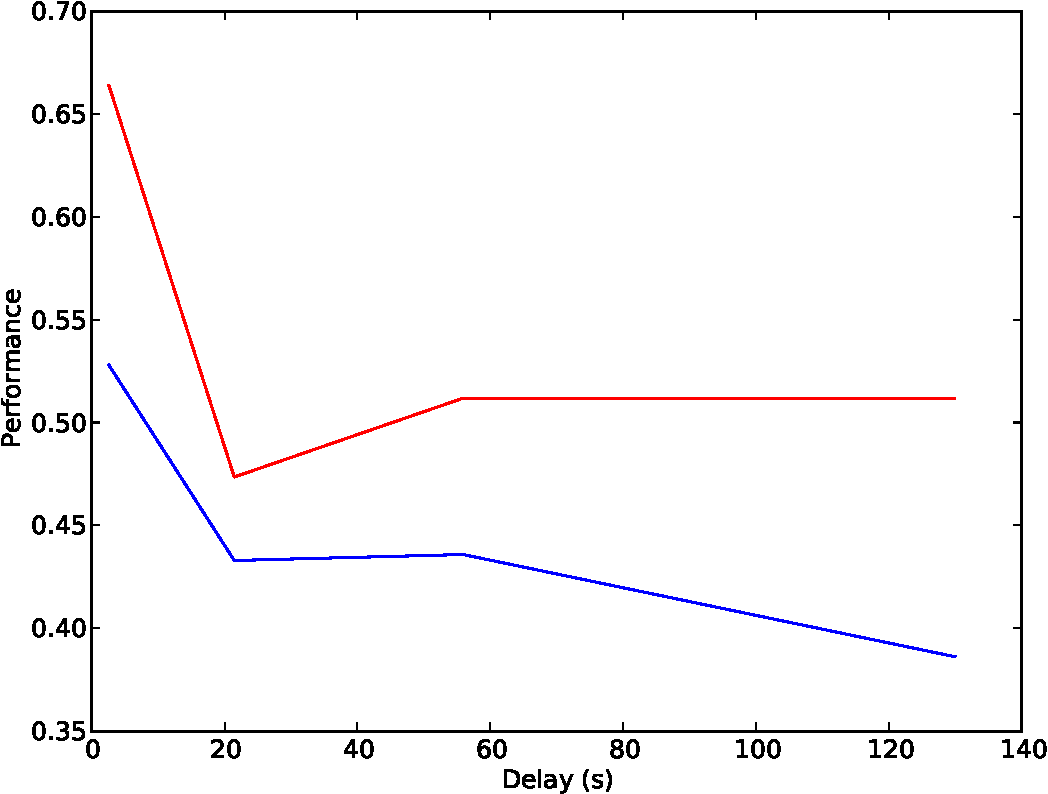
\includegraphics[width=0.4\textwidth]{figures/performance-verse-temporal-distance}
\caption{The average performance of the SVM and neural network classifiers plotted against the average temporal delay between data in the training and test sets.}
\label{fig:performance-verse-temporal-distance}
\end{figure}

The average confusion matrix presented in figure \ref{fig:average-confusion} gives a more intuitive look at the performance of the classifier.
From this matrix we can see that the classifiers are much better at detecting the presence of a single character than any other count.
In fact, there are almost no cases of confusion between 1 and 2 characters.
Apparently, these two situations evoke very different responses in the brain.
The rest of the character counts are distinguished with relatively equal accuracy.
However, there is a slight tendency to mis-classify the 6 character presentation.
It should also be noted that the majority of the incorrect responses lay just off the main diagonal.
These responses correspond to the classifier being wrong by a single character in its classification.
For example, the machine learning algorithm classified a frame as containing 4 characters when it only contained 3 characters.
The estimated performance does not take the cardinality of the classes into account and considers mislabeling 1 character as 2 equivalent to mislabeling 1 character as 6 characters.
A soft measure of accuracy that takes the cardinality of the classes into consideration may be useful but the results are harder to interpret.
A confusion matrix gives us the advantages of the soft measure while providing an easily interpretable look into the performance of the classifiers.

\begin{figure}
\centering
\begin{subfigure}{0.4\textwidth}
\centering

\begin{tabular}{*{9}{c}}
& & \multicolumn{6}{c}{predicted count} & \\
& & 1 & 2 & 3 & 4 & 5 & 6 & \\
\multirow{6}{*}{\begin{sideways}actual count\end{sideways}}
& 1 & \cellcolor[rgb]{0.000000,1.000000,0.000000}75\% & \cellcolor[rgb]{0.987315,0.012685,0.000000}6\% & \cellcolor[rgb]{0.967214,0.032786,0.000000}8\% & \cellcolor[rgb]{0.995154,0.004846,0.000000}3\% & \cellcolor[rgb]{0.996400,0.003600,0.000000}3\% & \cellcolor[rgb]{0.991856,0.008144,0.000000}5\% & \cellcolor[rgb]{0.000000,1.000000,0.000000}71\%\\
& 2 & \cellcolor[rgb]{0.984543,0.015457,0.000000}6\% & \cellcolor[rgb]{0.000001,0.999999,0.000000}52\% & \cellcolor[rgb]{0.960568,0.039432,0.000000}9\% & \cellcolor[rgb]{0.793233,0.206767,0.000000}13\% & \cellcolor[rgb]{0.989269,0.010731,0.000000}5\% & \cellcolor[rgb]{0.754492,0.245508,0.000000}14\% & \cellcolor[rgb]{0.000002,0.999998,0.000000}50\%\\
& 3 & \cellcolor[rgb]{0.976984,0.023016,0.000000}7\% & \cellcolor[rgb]{0.946464,0.053536,0.000000}9\% & \cellcolor[rgb]{0.000000,1.000000,0.000000}53\% & \cellcolor[rgb]{0.228780,0.771220,0.000000}20\% & \cellcolor[rgb]{0.980048,0.019952,0.000000}7\% & \cellcolor[rgb]{0.995294,0.004706,0.000000}3\% & \cellcolor[rgb]{0.000001,0.999999,0.000000}51\%\\
& 4 & \cellcolor[rgb]{0.992536,0.007464,0.000000}4\% & \cellcolor[rgb]{0.888490,0.111510,0.000000}11\% & \cellcolor[rgb]{0.154156,0.845844,0.000000}21\% & \cellcolor[rgb]{0.000336,0.999664,0.000000}37\% & \cellcolor[rgb]{0.500333,0.499667,0.000000}17\% & \cellcolor[rgb]{0.939464,0.060536,0.000000}10\% & \cellcolor[rgb]{0.000499,0.999501,0.000000}36\%\\
& 5 & \cellcolor[rgb]{0.995930,0.004070,0.000000}3\% & \cellcolor[rgb]{0.976984,0.023016,0.000000}7\% & \cellcolor[rgb]{0.934220,0.065780,0.000000}10\% & \cellcolor[rgb]{0.299381,0.700619,0.000000}19\% & \cellcolor[rgb]{0.000001,0.999999,0.000000}50\% & \cellcolor[rgb]{0.919415,0.080585,0.000000}11\% & \cellcolor[rgb]{0.000000,1.000000,0.000000}55\%\\
& 6 & \cellcolor[rgb]{0.917261,0.082739,0.000000}11\% & \cellcolor[rgb]{0.217071,0.782929,0.000000}20\% & \cellcolor[rgb]{0.994473,0.005527,0.000000}4\% & \cellcolor[rgb]{0.888730,0.111270,0.000000}11\% & \cellcolor[rgb]{0.880363,0.119637,0.000000}12\% & \cellcolor[rgb]{0.000031,0.999969,0.000000}43\% & \cellcolor[rgb]{0.000004,0.999996,0.000000}48\%\\
&   & \cellcolor[rgb]{0.000000,1.000000,0.000000}75\% & \cellcolor[rgb]{0.000001,0.999999,0.000000}52\% & \cellcolor[rgb]{0.000000,1.000000,0.000000}53\% & \cellcolor[rgb]{0.000336,0.999664,0.000000}37\% & \cellcolor[rgb]{0.000001,0.999999,0.000000}50\% & \cellcolor[rgb]{0.000031,0.999969,0.000000}43\% & \cellcolor[rgb]{0.000001,0.999999,0.000000}52\%\\
\end{tabular}

\caption{}
\label{fig:average-confusion-svm}
\end{subfigure}
\begin{subfigure}{0.4\textwidth}
\centering

\begin{tabular}{*{8}{c}}
& & \multicolumn{6}{c}{predicted count} \\
& & 1 & 2 & 3 & 4 & 5 & 6 \\
\multirow{6}{*}{\begin{sideways}actual count\end{sideways}}
& 1 & \cellcolor[rgb]{0.000000,1.000000,0.000000}62\% & \cellcolor[rgb]{0.975443,0.024557,0.000000}7\% & \cellcolor[rgb]{0.841309,0.158691,0.000000}12\% & \cellcolor[rgb]{0.971887,0.028113,0.000000}8\% & \cellcolor[rgb]{0.997938,0.002062,0.000000}1\% & \cellcolor[rgb]{0.960675,0.039325,0.000000}9\%\\
& 2 & \cellcolor[rgb]{0.933406,0.066594,0.000000}10\% & \cellcolor[rgb]{0.000009,0.999991,0.000000}46\% & \cellcolor[rgb]{0.933406,0.066594,0.000000}10\% & \cellcolor[rgb]{0.831816,0.168184,0.000000}13\% & \cellcolor[rgb]{0.989177,0.010823,0.000000}5\% & \cellcolor[rgb]{0.569328,0.430672,0.000000}16\%\\
& 3 & \cellcolor[rgb]{0.979969,0.020031,0.000000}7\% & \cellcolor[rgb]{0.960675,0.039325,0.000000}9\% & \cellcolor[rgb]{0.000018,0.999982,0.000000}44\% & \cellcolor[rgb]{0.071219,0.928781,0.000000}23\% & \cellcolor[rgb]{0.984753,0.015247,0.000000}6\% & \cellcolor[rgb]{0.902345,0.097655,0.000000}11\%\\
& 4 & \cellcolor[rgb]{0.989896,0.010104,0.000000}5\% & \cellcolor[rgb]{0.919227,0.080773,0.000000}11\% & \cellcolor[rgb]{0.159047,0.840953,0.000000}21\% & \cellcolor[rgb]{0.001187,0.998813,0.000000}34\% & \cellcolor[rgb]{0.739428,0.260572,0.000000}14\% & \cellcolor[rgb]{0.586267,0.413733,0.000000}16\%\\
& 5 & \cellcolor[rgb]{0.990567,0.009433,0.000000}5\% & \cellcolor[rgb]{0.971887,0.028113,0.000000}8\% & \cellcolor[rgb]{0.933406,0.066594,0.000000}10\% & \cellcolor[rgb]{0.333341,0.666659,0.000000}18\% & \cellcolor[rgb]{0.000017,0.999983,0.000000}44\% & \cellcolor[rgb]{0.697341,0.302659,0.000000}15\%\\
& 6 & \cellcolor[rgb]{0.945244,0.054756,0.000000}10\% & \cellcolor[rgb]{0.811482,0.188518,0.000000}13\% & \cellcolor[rgb]{0.937595,0.062405,0.000000}10\% & \cellcolor[rgb]{0.667251,0.332749,0.000000}15\% & \cellcolor[rgb]{0.902345,0.097655,0.000000}11\% & \cellcolor[rgb]{0.000049,0.999951,0.000000}41\%\\
\end{tabular}

\caption{}
\label{fig:average-confusion-nn}
\end{subfigure}
\caption{The average confusion matrices for the \subref{fig:average-confusion-svm} SVM and \subref{fig:average-confusion-nn} NN across all subjects using the block split.}
\label{fig:average-confusion}
\end{figure}

After aligning all of the subjects to the MNI template \ref{MNI} and combining these activation maps we found that the majority of activation took place in [need to do this analysis still].
This combined activation map is presented in figure \ref{fig:MNI-average-sensitivity}.

\begin{figure}
\centering
\begin{subfigure}{0.4\textwidth}
\centering
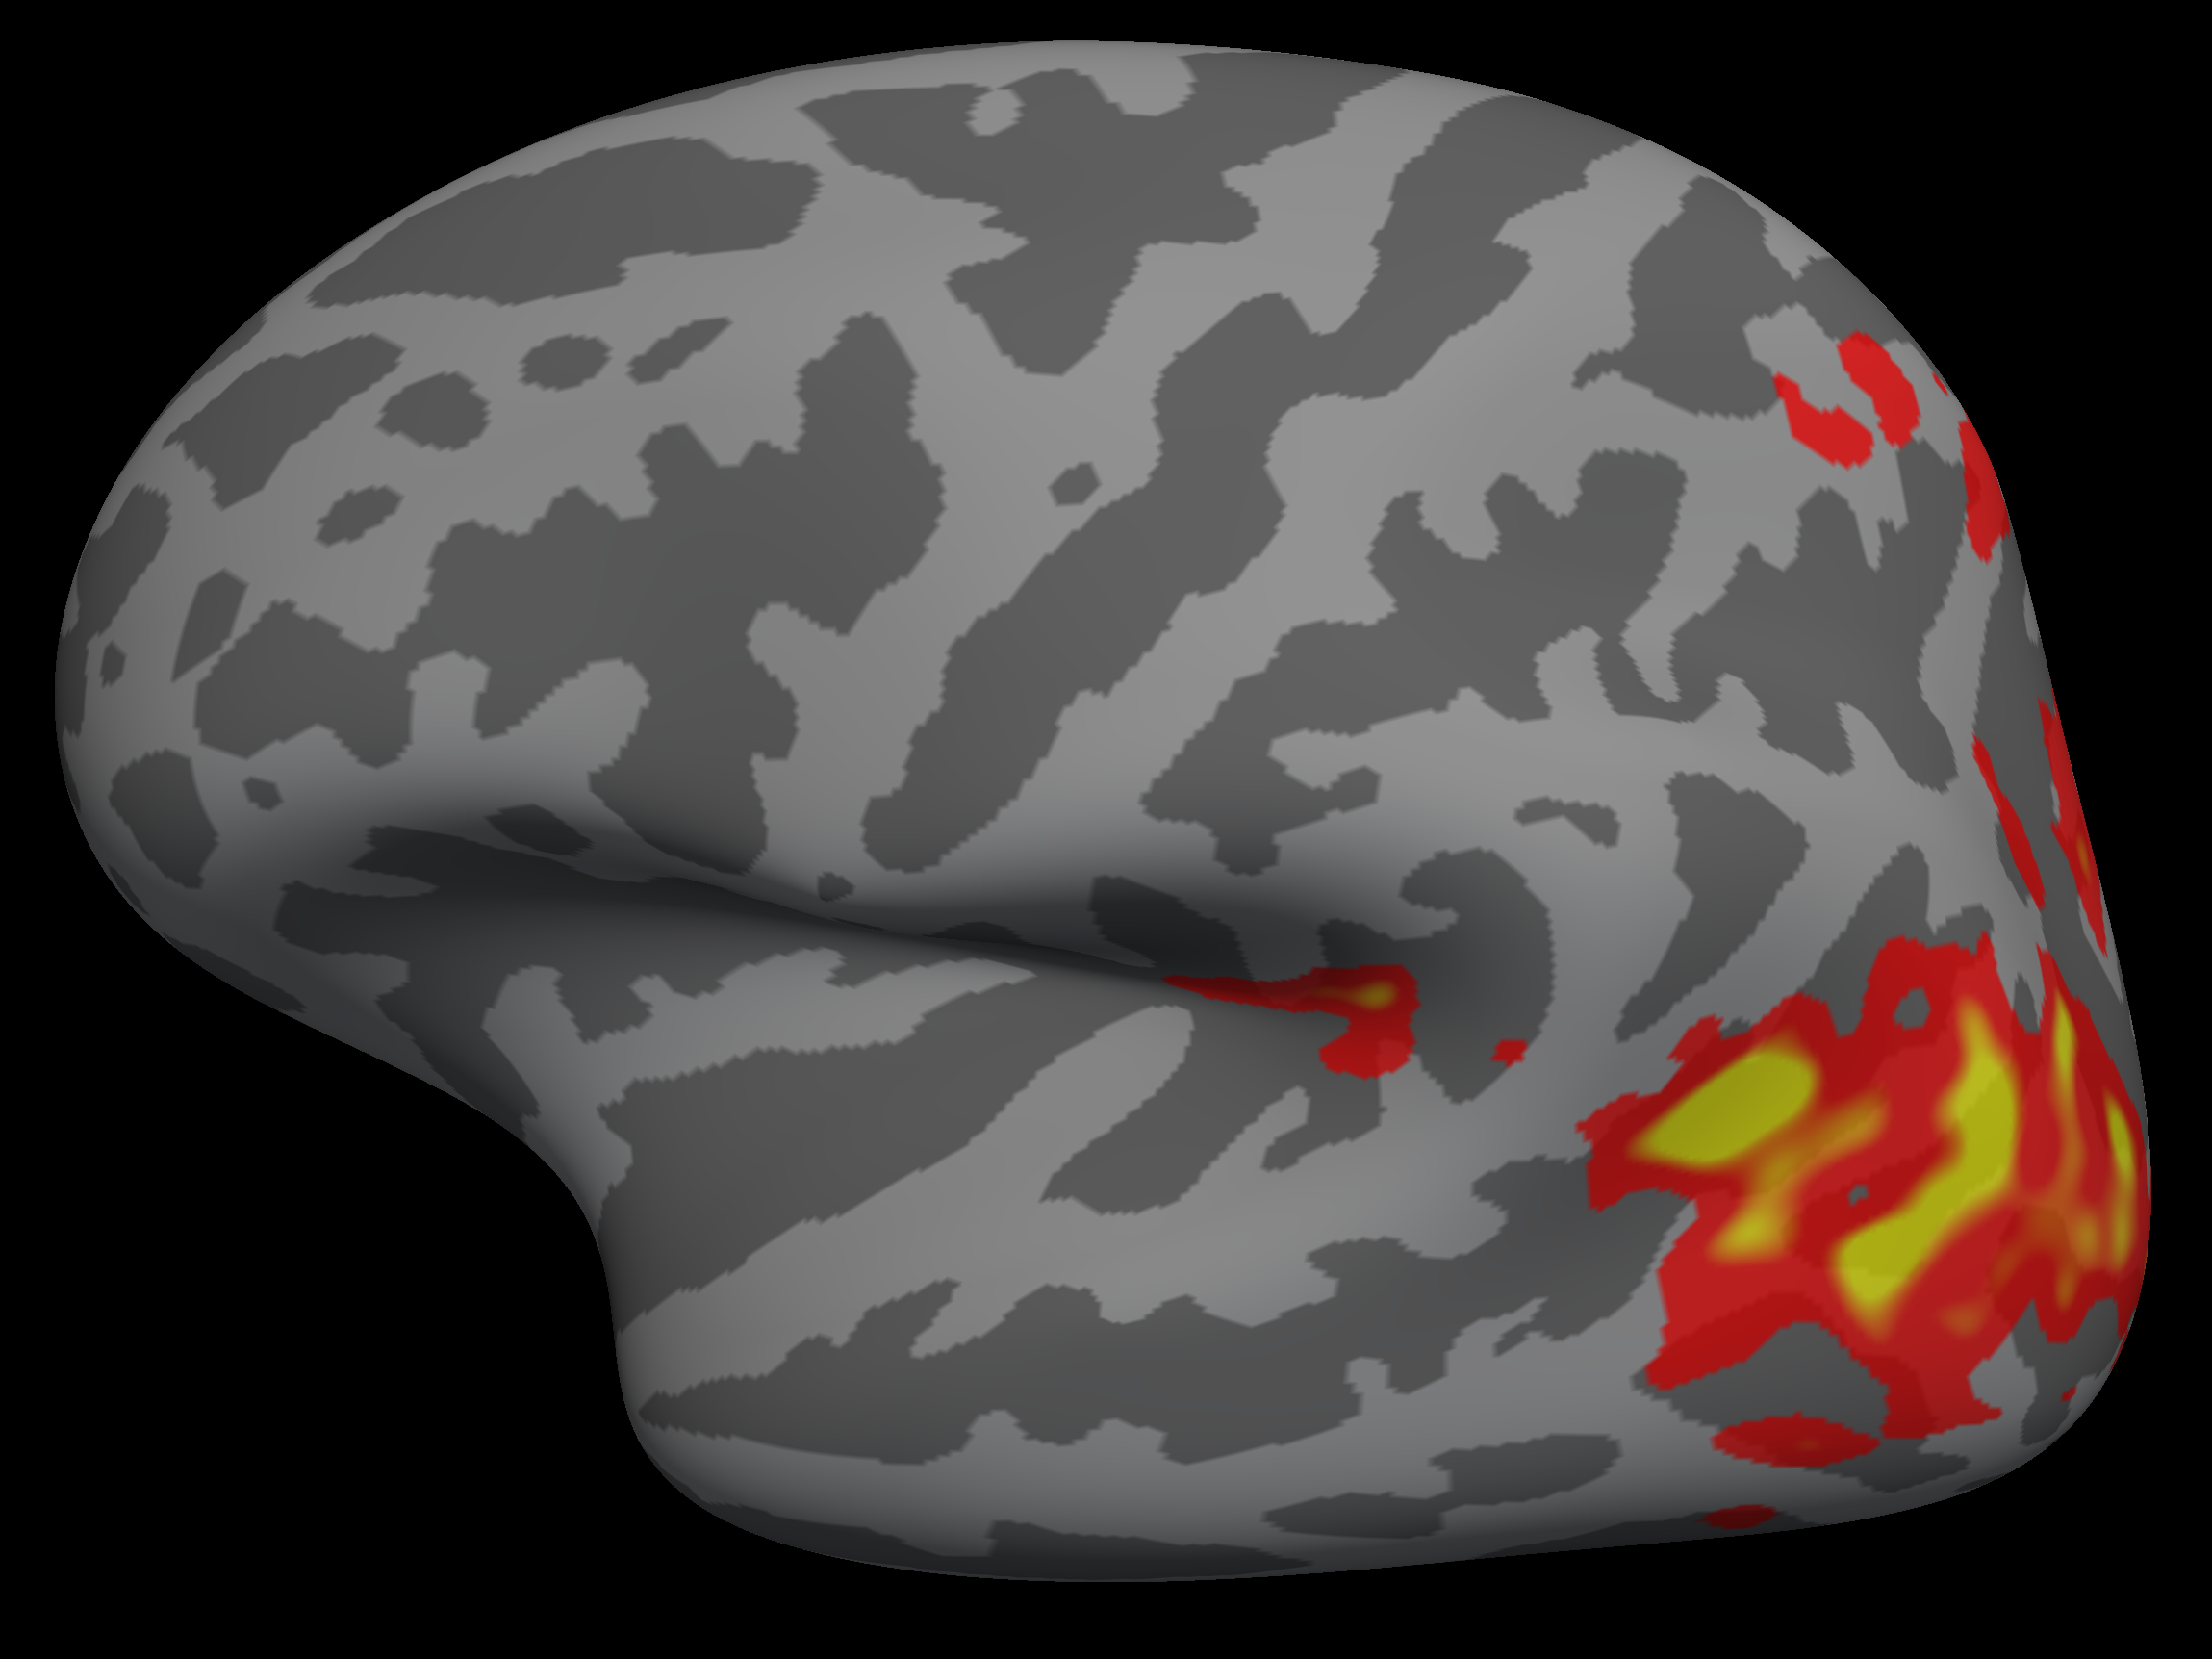
\includegraphics[width=\textwidth]{figures/lh-lateral-smax-average}
\caption{}
\label{fig:lh-lateral-smax-average}
\end{subfigure}
\begin{subfigure}{0.4\textwidth}
\centering
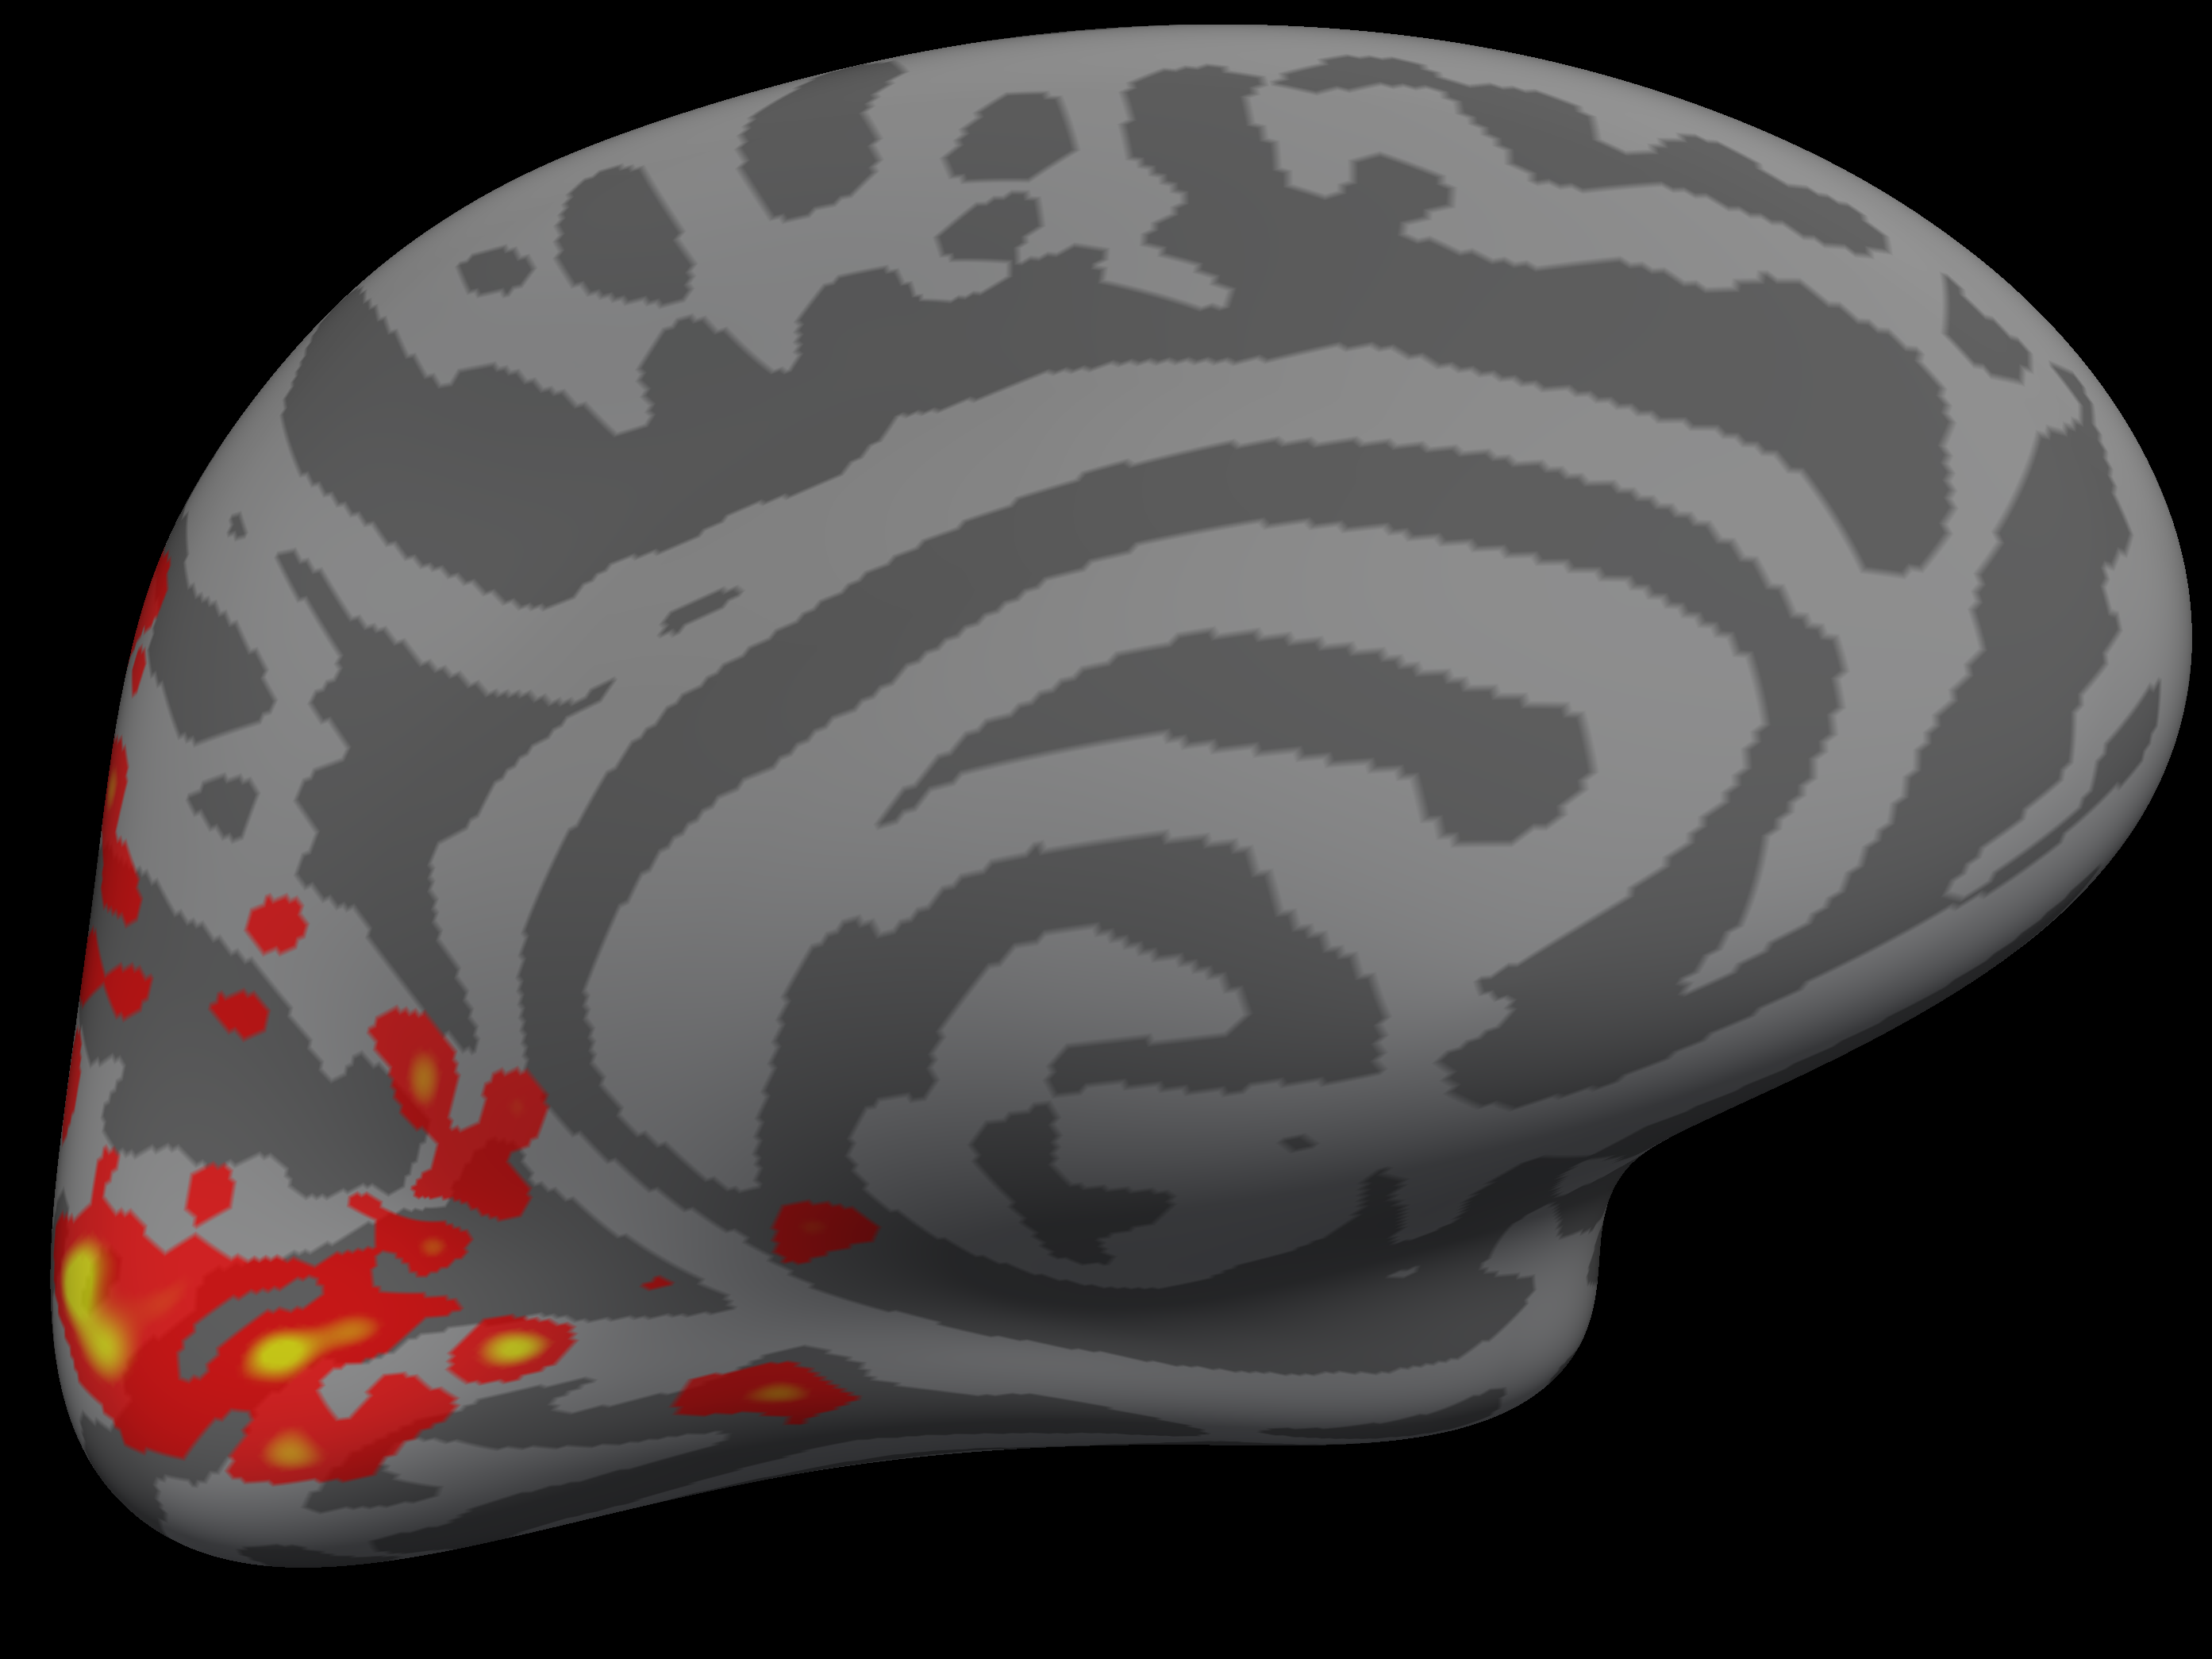
\includegraphics[width=\textwidth]{figures/lh-medial-smax-average}
\caption{}
\label{fig:lh-medial-smax-average}
\end{subfigure}
\begin{subfigure}{0.4\textwidth}
\centering
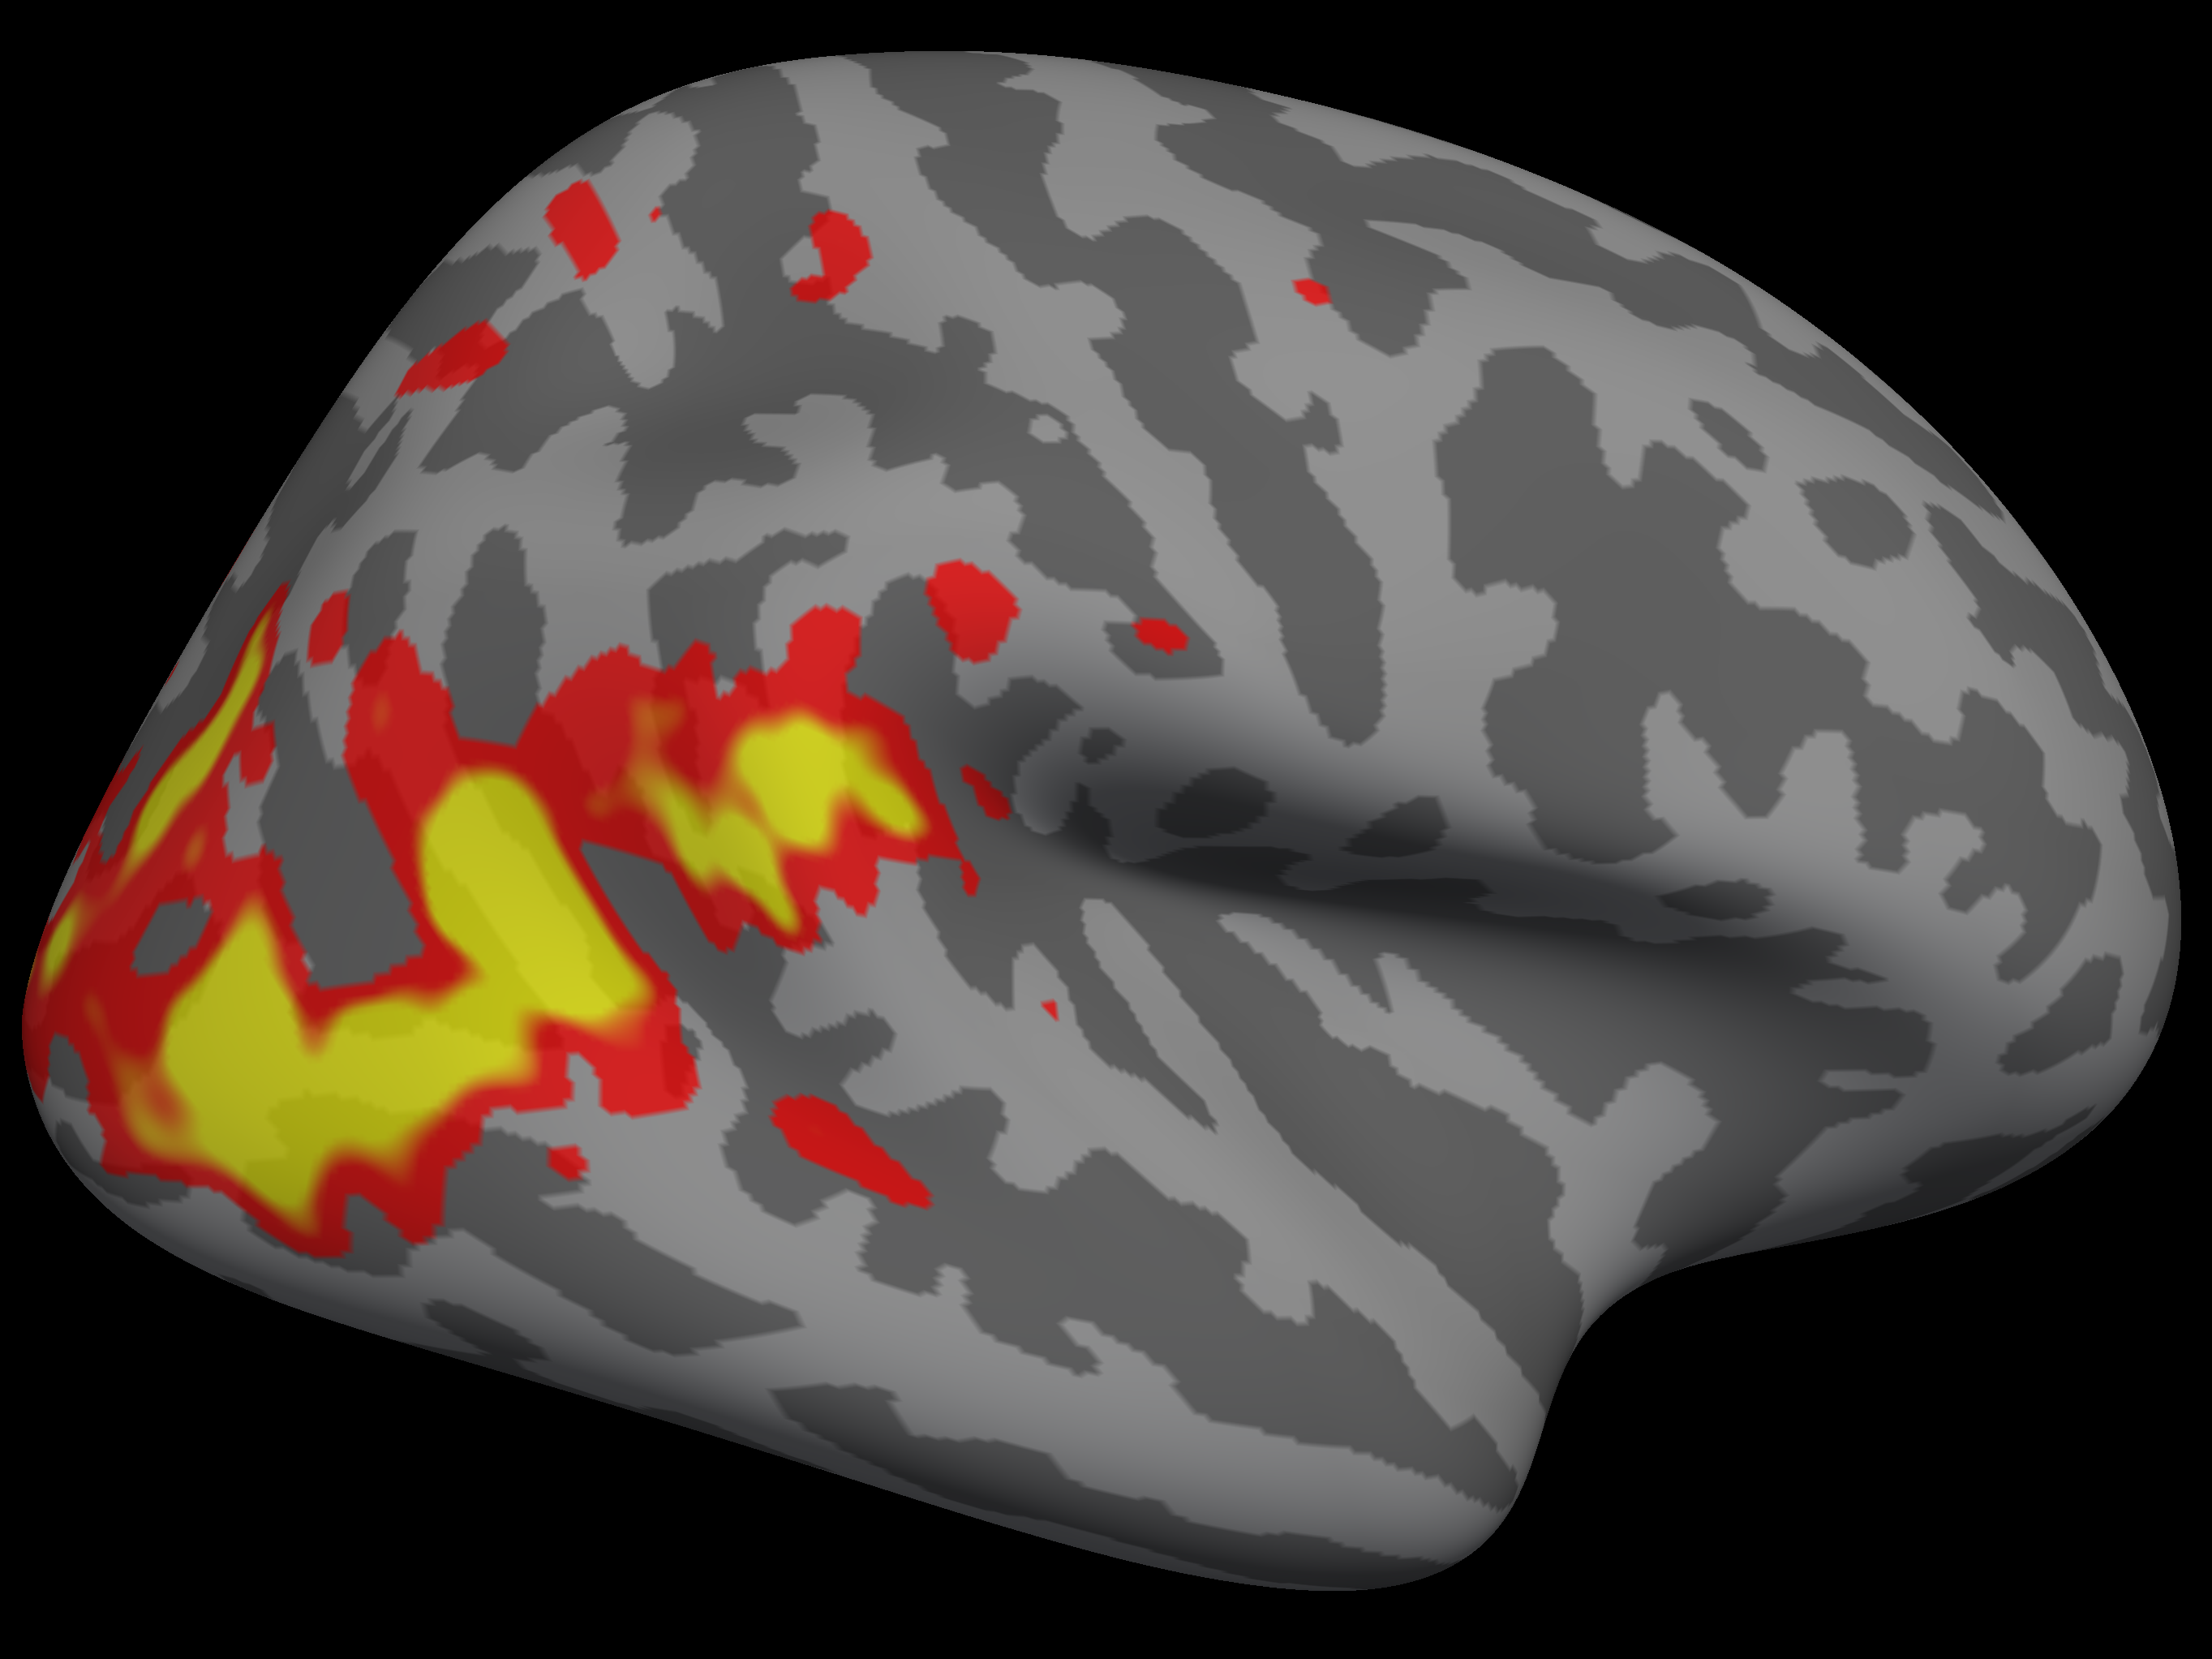
\includegraphics[width=\textwidth]{figures/rh-lateral-smax-average}
\caption{}
\label{fig:rh-lateral-smax-average}
\end{subfigure}
\begin{subfigure}{0.4\textwidth}
\centering
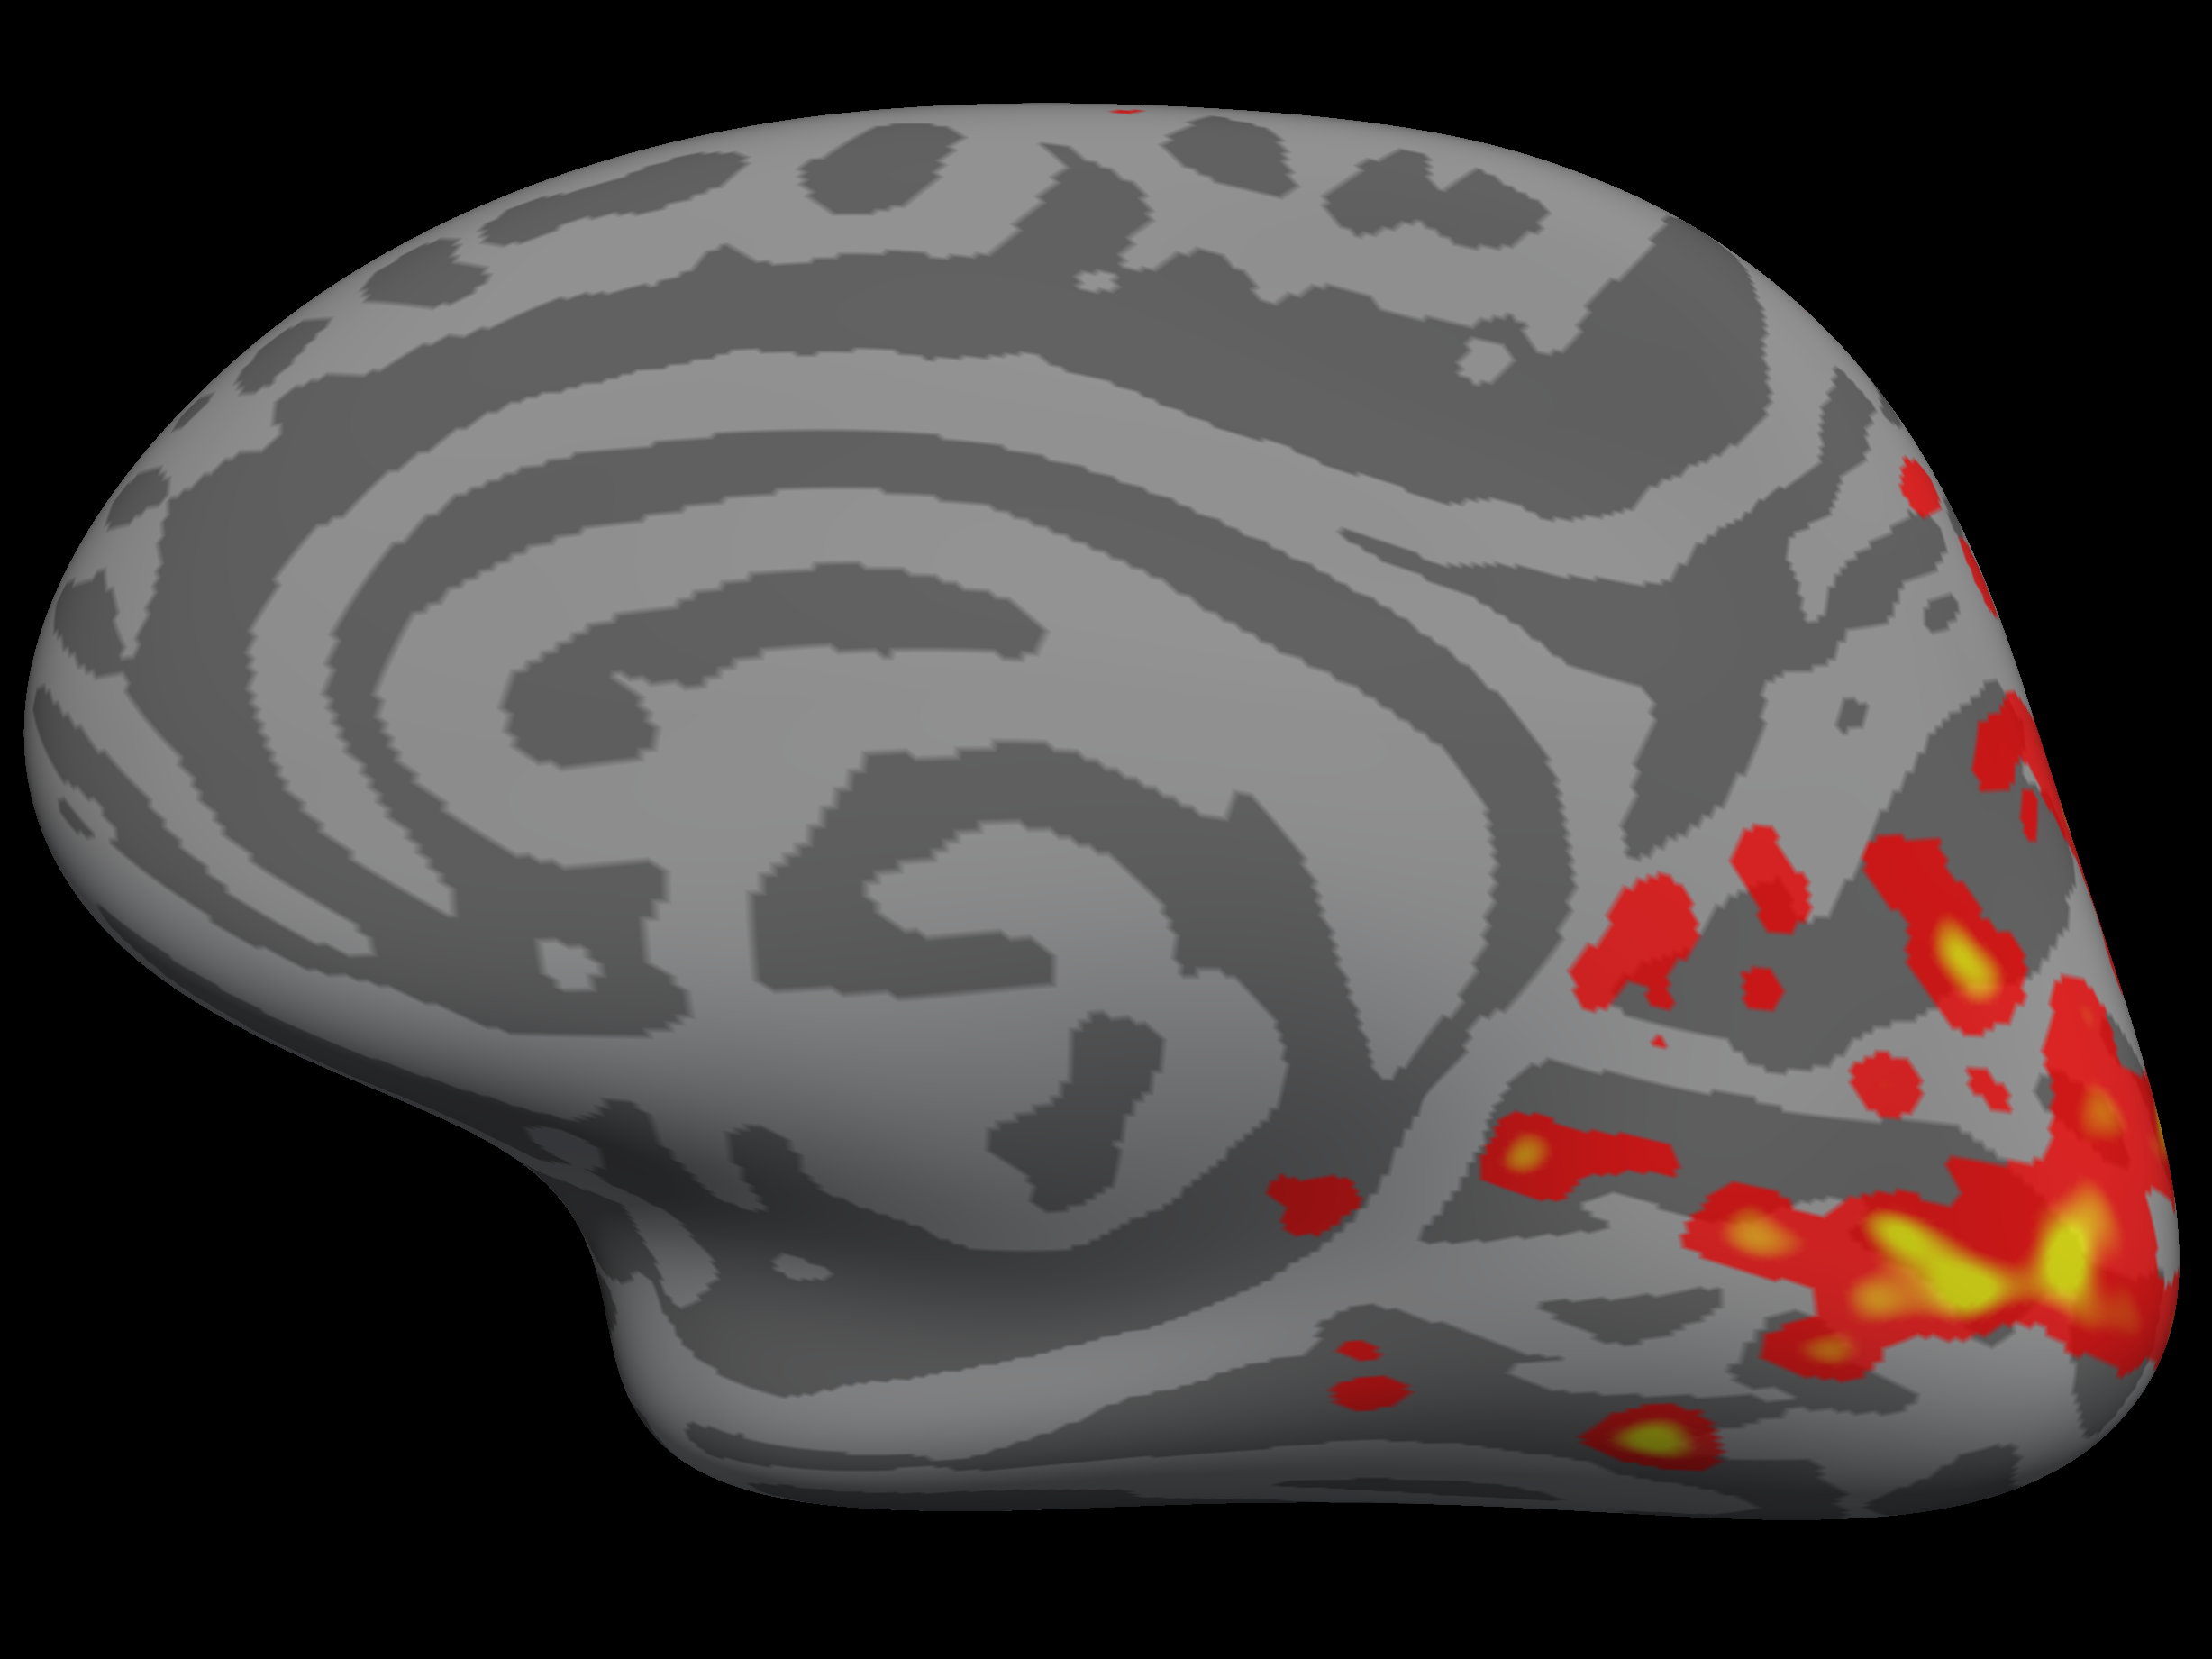
\includegraphics[width=\textwidth]{figures/rh-medial-smax-average}
\caption{}
\label{fig:rh-medial-smax-average}
\end{subfigure}
\caption{The sensitivity analysis agit veraged across all subjects mapped onto the slightly inflated MNI template brain.}
\label{fig:MNI-average-sensitivity}
\end{figure}

To better explore the relationship between sensitivity and classifier performance we plotted the performance of the classifier when trained on only a subset of the input voxels as determined by a minimum sensitivity cut off.
Figure \ref{fig:sensitivity-cutoff} shows this plot on top of the histogram of sensitivity values.
Interestingly, the performance of the classifier is not significantly affected until a majority of the voxels have been removed.
This would indicate that either only a small number of voxels are relevant for classification or that the information is highly redundant between voxels.
In actuality, it is likely a combination of the two.
The harmonic analysis will select some voxels that only appeared to covary with the stimulus presentation by chance.
These voxels will be assigned very low sensitivity values by the trained classifiers.
However, other voxels may actually covary with the stimulus but their patterns of activation may not be highly discriminative with respect to character count.
These voxels will also be assigned low sensitivity values by the trained classifiers.
Therefore, high sensitivity is sufficient but not necessary for the localization of a function in a particular region.

\begin{figure}
\centering
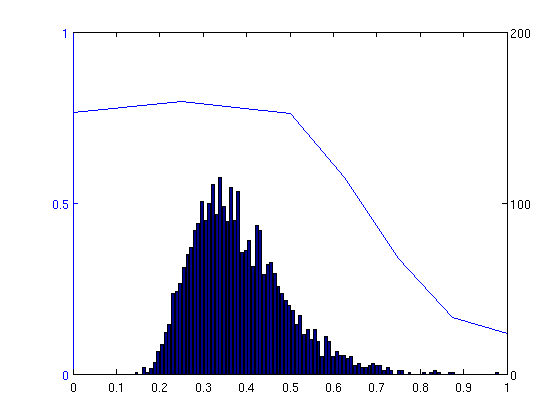
\includegraphics[width=0.4\textwidth]{figures/sensitivity-cutoff}
\caption{A histogram of the sensitivity analysis values and a plot of the feed forward neural network $F_1$ score when the inputs are pruned at a particular sensitivity value. }
\label{fig:sensitivity-cutoff}
\end{figure}

\section{Discussion}
Although both classifiers performed at well above chance levels for all subjects, the average performance on individual subjects varied significantly.
These variations could be the result of differences in age, general cognitive state, or simply how much attention the subject was paying to the stimulus during the scan.
The lack of a task during our stimulus makes these variations difficult to interpret since attention and cognitive state are not well controlled.
In future experiments, we plan to introduce a difficult task for the subjects to perform and we expect to see the average performance increase and the variation between subjects decrease.
However, the fact that the classifiers could still perform at well above chance levels without a focused task increases our confidence in the generalizability of the results of machine learning classifiers applied to fMRI data.


This could be a result of 6 characters being too much for the subject to consider individually.
Interestingly, the confusion is not often between 5 and 6 characters, but rather between 1 or 2 and 6 characters.
This would seem to indicate that when the number of characters grows too large, they are interpreted as a single unit.

The reported results are well above chance, indicating there is useful information about character number in the BOLD signal.
The sensitivity analysis indicates that no single region of the brain is responsible for counting characters, and there is not a simple linear relationship between magnitude of activation and cardinality.
Rather, it is a complex pattern of distributed activation requiring machine learning methods to capture the stimulus-response relationship.

Earlier, we presented this new trend in brain sate classification as a departure from traditional fMRI experiments which seek to identify the purpose or function of particular brain regions.
However, it is important to note that through sensitivity analysis these machine learning classifiers can be re-purposed for just that goal.
If a region of the brain is highly important for accurately predicting the presence of a particular stimulus then it logically follows that that region must somehow be involved in the processing of that stimulus.
Furthermore, multi-voxel non-linear machine learning classifiers can potentially identify much more complex interactions between brain regions than the simple GLM.

\bibliography{bib}

\end{document}
